% Created by tikzDevice version 0.12.3 on 2020-10-15 16:28:38
% !TEX encoding = UTF-8 Unicode
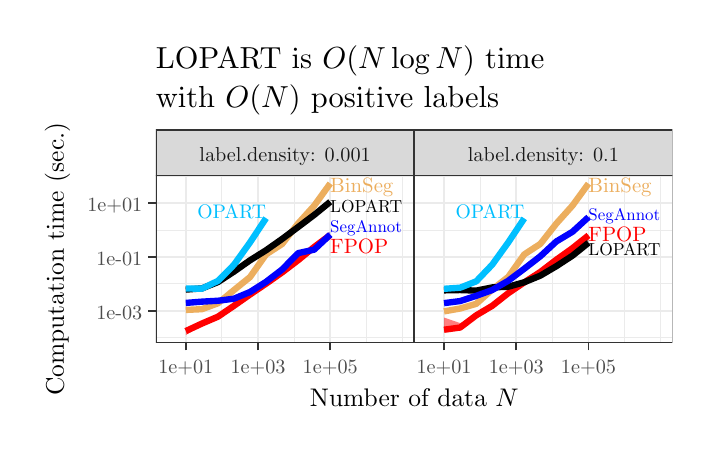
\begin{tikzpicture}[x=1pt,y=1pt]
\definecolor{fillColor}{RGB}{255,255,255}
\path[use as bounding box,fill=fillColor,fill opacity=0.00] (0,0) rectangle (238.49,144.54);
\begin{scope}
\path[clip] (  0.00,  0.00) rectangle (238.49,144.54);
\definecolor{drawColor}{RGB}{255,255,255}
\definecolor{fillColor}{RGB}{255,255,255}

\path[draw=drawColor,line width= 0.6pt,line join=round,line cap=round,fill=fillColor] ( -0.00,  0.00) rectangle (238.49,144.54);
\end{scope}
\begin{scope}
\path[clip] ( 46.36, 30.69) rectangle (139.68, 91.06);
\definecolor{fillColor}{RGB}{255,255,255}

\path[fill=fillColor] ( 46.36, 30.69) rectangle (139.68, 91.06);
\definecolor{drawColor}{gray}{0.92}

\path[draw=drawColor,line width= 0.3pt,line join=round] ( 46.36, 32.53) --
	(139.68, 32.53);

\path[draw=drawColor,line width= 0.3pt,line join=round] ( 46.36, 51.98) --
	(139.68, 51.98);

\path[draw=drawColor,line width= 0.3pt,line join=round] ( 46.36, 71.43) --
	(139.68, 71.43);

\path[draw=drawColor,line width= 0.3pt,line join=round] ( 46.36, 90.88) --
	(139.68, 90.88);

\path[draw=drawColor,line width= 0.3pt,line join=round] ( 70.18, 30.69) --
	( 70.18, 91.06);

\path[draw=drawColor,line width= 0.3pt,line join=round] ( 96.28, 30.69) --
	( 96.28, 91.06);

\path[draw=drawColor,line width= 0.3pt,line join=round] (122.39, 30.69) --
	(122.39, 91.06);

\path[draw=drawColor,line width= 0.3pt,line join=round] (135.44, 30.69) --
	(135.44, 91.06);

\path[draw=drawColor,line width= 0.6pt,line join=round] ( 46.36, 42.26) --
	(139.68, 42.26);

\path[draw=drawColor,line width= 0.6pt,line join=round] ( 46.36, 61.71) --
	(139.68, 61.71);

\path[draw=drawColor,line width= 0.6pt,line join=round] ( 46.36, 81.16) --
	(139.68, 81.16);

\path[draw=drawColor,line width= 0.6pt,line join=round] ( 57.13, 30.69) --
	( 57.13, 91.06);

\path[draw=drawColor,line width= 0.6pt,line join=round] ( 83.23, 30.69) --
	( 83.23, 91.06);

\path[draw=drawColor,line width= 0.6pt,line join=round] (109.33, 30.69) --
	(109.33, 91.06);
\definecolor{fillColor}{RGB}{236,174,94}

\path[fill=fillColor,fill opacity=0.50] ( 57.13, 42.80) --
	( 62.97, 43.29) --
	( 68.77, 45.12) --
	( 74.55, 49.85) --
	( 80.34, 54.47) --
	( 86.14, 62.62) --
	( 91.93, 66.42) --
	( 97.73, 73.82) --
	(103.53, 80.48) --
	(109.33, 88.31) --
	(109.33, 88.23) --
	(103.53, 80.19) --
	( 97.73, 73.78) --
	( 91.93, 66.32) --
	( 86.14, 62.59) --
	( 80.34, 54.29) --
	( 74.55, 49.71) --
	( 68.77, 44.82) --
	( 62.97, 42.55) --
	( 57.13, 42.32) --
	cycle;

\path[] ( 57.13, 42.80) --
	( 62.97, 43.29) --
	( 68.77, 45.12) --
	( 74.55, 49.85) --
	( 80.34, 54.47) --
	( 86.14, 62.62) --
	( 91.93, 66.42) --
	( 97.73, 73.82) --
	(103.53, 80.48) --
	(109.33, 88.31);

\path[] (109.33, 88.23) --
	(103.53, 80.19) --
	( 97.73, 73.78) --
	( 91.93, 66.32) --
	( 86.14, 62.59) --
	( 80.34, 54.29) --
	( 74.55, 49.71) --
	( 68.77, 44.82) --
	( 62.97, 42.55) --
	( 57.13, 42.32);
\definecolor{fillColor}{RGB}{255,0,0}

\path[fill=fillColor,fill opacity=0.50] ( 57.13, 35.51) --
	( 62.97, 37.72) --
	( 68.77, 40.58) --
	( 74.55, 44.42) --
	( 80.34, 48.36) --
	( 86.14, 52.58) --
	( 91.93, 56.16) --
	( 97.73, 60.63) --
	(103.53, 65.37) --
	(109.33, 69.82) --
	(109.33, 69.57) --
	(103.53, 65.03) --
	( 97.73, 60.48) --
	( 91.93, 56.07) --
	( 86.14, 51.87) --
	( 80.34, 47.99) --
	( 74.55, 43.99) --
	( 68.77, 39.68) --
	( 62.97, 37.08) --
	( 57.13, 33.43) --
	cycle;

\path[] ( 57.13, 35.51) --
	( 62.97, 37.72) --
	( 68.77, 40.58) --
	( 74.55, 44.42) --
	( 80.34, 48.36) --
	( 86.14, 52.58) --
	( 91.93, 56.16) --
	( 97.73, 60.63) --
	(103.53, 65.37) --
	(109.33, 69.82);

\path[] (109.33, 69.57) --
	(103.53, 65.03) --
	( 97.73, 60.48) --
	( 91.93, 56.07) --
	( 86.14, 51.87) --
	( 80.34, 47.99) --
	( 74.55, 43.99) --
	( 68.77, 39.68) --
	( 62.97, 37.08) --
	( 57.13, 33.43);
\definecolor{fillColor}{RGB}{0,0,0}

\path[fill=fillColor,fill opacity=0.50] ( 57.13, 50.24) --
	( 62.97, 50.41) --
	( 68.77, 52.88) --
	( 74.55, 56.44) --
	( 80.34, 60.50) --
	( 86.14, 64.30) --
	( 91.93, 68.19) --
	( 97.73, 72.59) --
	(103.53, 77.06) --
	(109.33, 81.65) --
	(109.33, 81.56) --
	(103.53, 76.73) --
	( 97.73, 72.50) --
	( 91.93, 68.17) --
	( 86.14, 64.09) --
	( 80.34, 60.46) --
	( 74.55, 56.32) --
	( 68.77, 52.50) --
	( 62.97, 49.83) --
	( 57.13, 49.89) --
	cycle;

\path[] ( 57.13, 50.24) --
	( 62.97, 50.41) --
	( 68.77, 52.88) --
	( 74.55, 56.44) --
	( 80.34, 60.50) --
	( 86.14, 64.30) --
	( 91.93, 68.19) --
	( 97.73, 72.59) --
	(103.53, 77.06) --
	(109.33, 81.65);

\path[] (109.33, 81.56) --
	(103.53, 76.73) --
	( 97.73, 72.50) --
	( 91.93, 68.17) --
	( 86.14, 64.09) --
	( 80.34, 60.46) --
	( 74.55, 56.32) --
	( 68.77, 52.50) --
	( 62.97, 49.83) --
	( 57.13, 49.89);
\definecolor{fillColor}{RGB}{0,191,255}

\path[fill=fillColor,fill opacity=0.50] ( 57.13, 50.61) --
	( 62.97, 50.29) --
	( 68.77, 53.17) --
	( 74.55, 58.92) --
	( 80.34, 66.97) --
	( 86.14, 75.83) --
	( 86.14, 75.65) --
	( 80.34, 66.91) --
	( 74.55, 58.83) --
	( 68.77, 52.87) --
	( 62.97, 50.03) --
	( 57.13, 49.78) --
	cycle;

\path[] ( 57.13, 50.61) --
	( 62.97, 50.29) --
	( 68.77, 53.17) --
	( 74.55, 58.92) --
	( 80.34, 66.97) --
	( 86.14, 75.83);

\path[] ( 86.14, 75.65) --
	( 80.34, 66.91) --
	( 74.55, 58.83) --
	( 68.77, 52.87) --
	( 62.97, 50.03) --
	( 57.13, 49.78);
\definecolor{fillColor}{RGB}{0,0,255}

\path[fill=fillColor,fill opacity=0.50] ( 57.13, 45.09) --
	( 62.97, 45.91) --
	( 68.77, 45.86) --
	( 74.55, 47.50) --
	( 80.34, 49.20) --
	( 86.14, 53.56) --
	( 91.93, 57.15) --
	( 97.73, 63.68) --
	(103.53, 64.61) --
	(109.33, 70.89) --
	(109.33, 69.46) --
	(103.53, 64.31) --
	( 97.73, 63.02) --
	( 91.93, 57.14) --
	( 86.14, 52.22) --
	( 80.34, 48.97) --
	( 74.55, 46.42) --
	( 68.77, 45.28) --
	( 62.97, 44.75) --
	( 57.13, 44.21) --
	cycle;

\path[] ( 57.13, 45.09) --
	( 62.97, 45.91) --
	( 68.77, 45.86) --
	( 74.55, 47.50) --
	( 80.34, 49.20) --
	( 86.14, 53.56) --
	( 91.93, 57.15) --
	( 97.73, 63.68) --
	(103.53, 64.61) --
	(109.33, 70.89);

\path[] (109.33, 69.46) --
	(103.53, 64.31) --
	( 97.73, 63.02) --
	( 91.93, 57.14) --
	( 86.14, 52.22) --
	( 80.34, 48.97) --
	( 74.55, 46.42) --
	( 68.77, 45.28) --
	( 62.97, 44.75) --
	( 57.13, 44.21);
\definecolor{drawColor}{RGB}{236,174,94}

\path[draw=drawColor,line width= 2.3pt,line join=round] ( 57.13, 42.55) --
	( 62.97, 42.82) --
	( 68.77, 44.95) --
	( 74.55, 49.73) --
	( 80.34, 54.41) --
	( 86.14, 62.61) --
	( 91.93, 66.36) --
	( 97.73, 73.80) --
	(103.53, 80.21) --
	(109.33, 88.23);
\definecolor{drawColor}{RGB}{255,0,0}

\path[draw=drawColor,line width= 2.3pt,line join=round] ( 57.13, 34.90) --
	( 62.97, 37.63) --
	( 68.77, 40.11) --
	( 74.55, 44.05) --
	( 80.34, 48.11) --
	( 86.14, 52.03) --
	( 91.93, 56.10) --
	( 97.73, 60.51) --
	(103.53, 65.29) --
	(109.33, 69.62);
\definecolor{drawColor}{RGB}{0,0,0}

\path[draw=drawColor,line width= 2.3pt,line join=round] ( 57.13, 49.90) --
	( 62.97, 50.32) --
	( 68.77, 52.62) --
	( 74.55, 56.39) --
	( 80.34, 60.47) --
	( 86.14, 64.11) --
	( 91.93, 68.18) --
	( 97.73, 72.50) --
	(103.53, 76.88) --
	(109.33, 81.62);
\definecolor{drawColor}{RGB}{0,191,255}

\path[draw=drawColor,line width= 2.3pt,line join=round] ( 57.13, 50.29) --
	( 62.97, 50.23) --
	( 68.77, 53.05) --
	( 74.55, 58.87) --
	( 80.34, 66.93) --
	( 86.14, 75.70);
\definecolor{drawColor}{RGB}{0,0,255}

\path[draw=drawColor,line width= 2.3pt,line join=round] ( 57.13, 45.08) --
	( 62.97, 45.54) --
	( 68.77, 45.86) --
	( 74.55, 46.61) --
	( 80.34, 49.03) --
	( 86.14, 52.70) --
	( 91.93, 57.15) --
	( 97.73, 63.07) --
	(103.53, 64.33) --
	(109.33, 69.77);
\end{scope}
\begin{scope}
\path[clip] ( 46.36, 30.69) rectangle (139.68, 91.06);
\definecolor{drawColor}{RGB}{255,0,0}

\node[text=drawColor,anchor=base west,inner sep=0pt, outer sep=0pt, scale=  0.75] at (109.33, 63.09) {FPOP};
\definecolor{drawColor}{RGB}{0,0,255}

\node[text=drawColor,anchor=base west,inner sep=0pt, outer sep=0pt, scale=  0.61] at (109.33, 70.70) {SegAnnot};
\definecolor{drawColor}{RGB}{0,0,0}

\node[text=drawColor,anchor=base west,inner sep=0pt, outer sep=0pt, scale=  0.63] at (109.33, 77.93) {LOPART};
\definecolor{drawColor}{RGB}{236,174,94}

\node[text=drawColor,anchor=base west,inner sep=0pt, outer sep=0pt, scale=  0.75] at (109.33, 84.86) {BinSeg};
\definecolor{drawColor}{RGB}{0,191,255}

\node[text=drawColor,anchor=base east,inner sep=0pt, outer sep=0pt, scale=  0.71] at ( 86.14, 75.70) {OPART};
\definecolor{drawColor}{gray}{0.20}

\path[draw=drawColor,line width= 0.6pt,line join=round,line cap=round] ( 46.36, 30.69) rectangle (139.68, 91.06);
\end{scope}
\begin{scope}
\path[clip] (139.68, 30.69) rectangle (232.99, 91.06);
\definecolor{fillColor}{RGB}{255,255,255}

\path[fill=fillColor] (139.68, 30.69) rectangle (232.99, 91.06);
\definecolor{drawColor}{gray}{0.92}

\path[draw=drawColor,line width= 0.3pt,line join=round] (139.68, 32.53) --
	(232.99, 32.53);

\path[draw=drawColor,line width= 0.3pt,line join=round] (139.68, 51.98) --
	(232.99, 51.98);

\path[draw=drawColor,line width= 0.3pt,line join=round] (139.68, 71.43) --
	(232.99, 71.43);

\path[draw=drawColor,line width= 0.3pt,line join=round] (139.68, 90.88) --
	(232.99, 90.88);

\path[draw=drawColor,line width= 0.3pt,line join=round] (163.50, 30.69) --
	(163.50, 91.06);

\path[draw=drawColor,line width= 0.3pt,line join=round] (189.60, 30.69) --
	(189.60, 91.06);

\path[draw=drawColor,line width= 0.3pt,line join=round] (215.70, 30.69) --
	(215.70, 91.06);

\path[draw=drawColor,line width= 0.3pt,line join=round] (228.75, 30.69) --
	(228.75, 91.06);

\path[draw=drawColor,line width= 0.6pt,line join=round] (139.68, 42.26) --
	(232.99, 42.26);

\path[draw=drawColor,line width= 0.6pt,line join=round] (139.68, 61.71) --
	(232.99, 61.71);

\path[draw=drawColor,line width= 0.6pt,line join=round] (139.68, 81.16) --
	(232.99, 81.16);

\path[draw=drawColor,line width= 0.6pt,line join=round] (150.44, 30.69) --
	(150.44, 91.06);

\path[draw=drawColor,line width= 0.6pt,line join=round] (176.55, 30.69) --
	(176.55, 91.06);

\path[draw=drawColor,line width= 0.6pt,line join=round] (202.65, 30.69) --
	(202.65, 91.06);
\definecolor{fillColor}{RGB}{236,174,94}

\path[fill=fillColor,fill opacity=0.50] (150.44, 43.02) --
	(156.28, 43.16) --
	(162.09, 44.94) --
	(167.86, 49.91) --
	(173.65, 54.49) --
	(179.45, 62.70) --
	(185.25, 66.42) --
	(191.05, 73.85) --
	(196.85, 80.26) --
	(202.65, 88.19) --
	(202.65, 88.14) --
	(196.85, 80.21) --
	(191.05, 73.73) --
	(185.25, 66.35) --
	(179.45, 62.62) --
	(173.65, 54.34) --
	(167.86, 49.80) --
	(162.09, 44.49) --
	(156.28, 42.63) --
	(150.44, 41.63) --
	cycle;

\path[] (150.44, 43.02) --
	(156.28, 43.16) --
	(162.09, 44.94) --
	(167.86, 49.91) --
	(173.65, 54.49) --
	(179.45, 62.70) --
	(185.25, 66.42) --
	(191.05, 73.85) --
	(196.85, 80.26) --
	(202.65, 88.19);

\path[] (202.65, 88.14) --
	(196.85, 80.21) --
	(191.05, 73.73) --
	(185.25, 66.35) --
	(179.45, 62.62) --
	(173.65, 54.34) --
	(167.86, 49.80) --
	(162.09, 44.49) --
	(156.28, 42.63) --
	(150.44, 41.63);
\definecolor{fillColor}{RGB}{255,0,0}

\path[fill=fillColor,fill opacity=0.50] (150.44, 39.80) --
	(156.28, 37.79) --
	(162.09, 40.65) --
	(167.86, 44.48) --
	(173.65, 48.59) --
	(179.45, 52.53) --
	(185.25, 56.42) --
	(191.05, 60.91) --
	(196.85, 64.86) --
	(202.65, 69.79) --
	(202.65, 69.41) --
	(196.85, 64.84) --
	(191.05, 60.67) --
	(185.25, 56.25) --
	(179.45, 52.44) --
	(173.65, 48.41) --
	(167.86, 43.88) --
	(162.09, 40.48) --
	(156.28, 35.87) --
	(150.44, 34.61) --
	cycle;

\path[] (150.44, 39.80) --
	(156.28, 37.79) --
	(162.09, 40.65) --
	(167.86, 44.48) --
	(173.65, 48.59) --
	(179.45, 52.53) --
	(185.25, 56.42) --
	(191.05, 60.91) --
	(196.85, 64.86) --
	(202.65, 69.79);

\path[] (202.65, 69.41) --
	(196.85, 64.84) --
	(191.05, 60.67) --
	(185.25, 56.25) --
	(179.45, 52.44) --
	(173.65, 48.41) --
	(167.86, 43.88) --
	(162.09, 40.48) --
	(156.28, 35.87) --
	(150.44, 34.61);
\definecolor{fillColor}{RGB}{0,0,0}

\path[fill=fillColor,fill opacity=0.50] (150.44, 49.97) --
	(156.28, 49.73) --
	(162.09, 49.59) --
	(167.86, 50.74) --
	(173.65, 50.94) --
	(179.45, 52.82) --
	(185.25, 55.11) --
	(191.05, 58.43) --
	(196.85, 62.48) --
	(202.65, 68.93) --
	(202.65, 66.65) --
	(196.85, 62.12) --
	(191.05, 58.22) --
	(185.25, 54.93) --
	(179.45, 52.55) --
	(173.65, 50.83) --
	(167.86, 50.14) --
	(162.09, 49.46) --
	(156.28, 49.47) --
	(150.44, 49.29) --
	cycle;

\path[] (150.44, 49.97) --
	(156.28, 49.73) --
	(162.09, 49.59) --
	(167.86, 50.74) --
	(173.65, 50.94) --
	(179.45, 52.82) --
	(185.25, 55.11) --
	(191.05, 58.43) --
	(196.85, 62.48) --
	(202.65, 68.93);

\path[] (202.65, 66.65) --
	(196.85, 62.12) --
	(191.05, 58.22) --
	(185.25, 54.93) --
	(179.45, 52.55) --
	(173.65, 50.83) --
	(167.86, 50.14) --
	(162.09, 49.46) --
	(156.28, 49.47) --
	(150.44, 49.29);
\definecolor{fillColor}{RGB}{0,191,255}

\path[fill=fillColor,fill opacity=0.50] (150.44, 50.23) --
	(156.28, 51.06) --
	(162.09, 53.16) --
	(167.86, 58.97) --
	(173.65, 66.93) --
	(179.45, 75.65) --
	(179.45, 75.58) --
	(173.65, 66.92) --
	(167.86, 58.87) --
	(162.09, 52.62) --
	(156.28, 50.55) --
	(150.44, 49.97) --
	cycle;

\path[] (150.44, 50.23) --
	(156.28, 51.06) --
	(162.09, 53.16) --
	(167.86, 58.97) --
	(173.65, 66.93) --
	(179.45, 75.65);

\path[] (179.45, 75.58) --
	(173.65, 66.92) --
	(167.86, 58.87) --
	(162.09, 52.62) --
	(156.28, 50.55) --
	(150.44, 49.97);
\definecolor{fillColor}{RGB}{0,0,255}

\path[fill=fillColor,fill opacity=0.50] (150.44, 45.75) --
	(156.28, 45.92) --
	(162.09, 47.87) --
	(167.86, 49.92) --
	(173.65, 53.17) --
	(179.45, 57.56) --
	(185.25, 61.97) --
	(191.05, 67.37) --
	(196.85, 70.77) --
	(202.65, 76.23) --
	(202.65, 76.06) --
	(196.85, 70.67) --
	(191.05, 67.26) --
	(185.25, 61.78) --
	(179.45, 57.40) --
	(173.65, 52.96) --
	(167.86, 49.69) --
	(162.09, 47.17) --
	(156.28, 45.45) --
	(150.44, 44.56) --
	cycle;

\path[] (150.44, 45.75) --
	(156.28, 45.92) --
	(162.09, 47.87) --
	(167.86, 49.92) --
	(173.65, 53.17) --
	(179.45, 57.56) --
	(185.25, 61.97) --
	(191.05, 67.37) --
	(196.85, 70.77) --
	(202.65, 76.23);

\path[] (202.65, 76.06) --
	(196.85, 70.67) --
	(191.05, 67.26) --
	(185.25, 61.78) --
	(179.45, 57.40) --
	(173.65, 52.96) --
	(167.86, 49.69) --
	(162.09, 47.17) --
	(156.28, 45.45) --
	(150.44, 44.56);
\definecolor{drawColor}{RGB}{236,174,94}

\path[draw=drawColor,line width= 2.3pt,line join=round] (150.44, 42.02) --
	(156.28, 43.06) --
	(162.09, 44.75) --
	(167.86, 49.91) --
	(173.65, 54.48) --
	(179.45, 62.62) --
	(185.25, 66.40) --
	(191.05, 73.77) --
	(196.85, 80.23) --
	(202.65, 88.18);
\definecolor{drawColor}{RGB}{255,0,0}

\path[draw=drawColor,line width= 2.3pt,line join=round] (150.44, 35.39) --
	(156.28, 36.19) --
	(162.09, 40.60) --
	(167.86, 44.03) --
	(173.65, 48.58) --
	(179.45, 52.51) --
	(185.25, 56.27) --
	(191.05, 60.70) --
	(196.85, 64.85) --
	(202.65, 69.48);
\definecolor{drawColor}{RGB}{0,0,0}

\path[draw=drawColor,line width= 2.3pt,line join=round] (150.44, 49.62) --
	(156.28, 49.73) --
	(162.09, 49.53) --
	(167.86, 50.68) --
	(173.65, 50.93) --
	(179.45, 52.55) --
	(185.25, 54.94) --
	(191.05, 58.36) --
	(196.85, 62.14) --
	(202.65, 66.80);
\definecolor{drawColor}{RGB}{0,191,255}

\path[draw=drawColor,line width= 2.3pt,line join=round] (150.44, 50.18) --
	(156.28, 50.58) --
	(162.09, 52.88) --
	(167.86, 58.90) --
	(173.65, 66.93) --
	(179.45, 75.62);
\definecolor{drawColor}{RGB}{0,0,255}

\path[draw=drawColor,line width= 2.3pt,line join=round] (150.44, 45.00) --
	(156.28, 45.75) --
	(162.09, 47.64) --
	(167.86, 49.74) --
	(173.65, 53.08) --
	(179.45, 57.44) --
	(185.25, 61.93) --
	(191.05, 67.30) --
	(196.85, 70.77) --
	(202.65, 76.08);
\end{scope}
\begin{scope}
\path[clip] (139.68, 30.69) rectangle (232.99, 91.06);
\definecolor{drawColor}{RGB}{0,0,0}

\node[text=drawColor,anchor=base west,inner sep=0pt, outer sep=0pt, scale=  0.63] at (202.65, 62.07) {LOPART};
\definecolor{drawColor}{RGB}{255,0,0}

\node[text=drawColor,anchor=base west,inner sep=0pt, outer sep=0pt, scale=  0.75] at (202.65, 67.24) {FPOP};
\definecolor{drawColor}{RGB}{0,0,255}

\node[text=drawColor,anchor=base west,inner sep=0pt, outer sep=0pt, scale=  0.61] at (202.65, 74.86) {SegAnnot};
\definecolor{drawColor}{RGB}{236,174,94}

\node[text=drawColor,anchor=base west,inner sep=0pt, outer sep=0pt, scale=  0.75] at (202.65, 84.86) {BinSeg};
\definecolor{drawColor}{RGB}{0,191,255}

\node[text=drawColor,anchor=base east,inner sep=0pt, outer sep=0pt, scale=  0.71] at (179.45, 75.62) {OPART};
\definecolor{drawColor}{gray}{0.20}

\path[draw=drawColor,line width= 0.6pt,line join=round,line cap=round] (139.68, 30.69) rectangle (232.99, 91.06);
\end{scope}
\begin{scope}
\path[clip] ( 46.36, 91.06) rectangle (139.68,107.63);
\definecolor{drawColor}{gray}{0.20}
\definecolor{fillColor}{gray}{0.85}

\path[draw=drawColor,line width= 0.6pt,line join=round,line cap=round,fill=fillColor] ( 46.36, 91.06) rectangle (139.68,107.63);
\definecolor{drawColor}{gray}{0.10}

\node[text=drawColor,anchor=base,inner sep=0pt, outer sep=0pt, scale=  0.73] at ( 93.02, 96.31) {label.density: 0.001};
\end{scope}
\begin{scope}
\path[clip] (139.68, 91.06) rectangle (232.99,107.63);
\definecolor{drawColor}{gray}{0.20}
\definecolor{fillColor}{gray}{0.85}

\path[draw=drawColor,line width= 0.6pt,line join=round,line cap=round,fill=fillColor] (139.68, 91.06) rectangle (232.99,107.63);
\definecolor{drawColor}{gray}{0.10}

\node[text=drawColor,anchor=base,inner sep=0pt, outer sep=0pt, scale=  0.73] at (186.33, 96.31) {label.density: 0.1};
\end{scope}
\begin{scope}
\path[clip] (  0.00,  0.00) rectangle (238.49,144.54);
\definecolor{drawColor}{gray}{0.20}

\path[draw=drawColor,line width= 0.6pt,line join=round] ( 57.13, 27.94) --
	( 57.13, 30.69);

\path[draw=drawColor,line width= 0.6pt,line join=round] ( 83.23, 27.94) --
	( 83.23, 30.69);

\path[draw=drawColor,line width= 0.6pt,line join=round] (109.33, 27.94) --
	(109.33, 30.69);
\end{scope}
\begin{scope}
\path[clip] (  0.00,  0.00) rectangle (238.49,144.54);
\definecolor{drawColor}{gray}{0.30}

\node[text=drawColor,anchor=base,inner sep=0pt, outer sep=0pt, scale=  0.73] at ( 57.13, 19.68) {1e+01};

\node[text=drawColor,anchor=base,inner sep=0pt, outer sep=0pt, scale=  0.73] at ( 83.23, 19.68) {1e+03};

\node[text=drawColor,anchor=base,inner sep=0pt, outer sep=0pt, scale=  0.73] at (109.33, 19.68) {1e+05};
\end{scope}
\begin{scope}
\path[clip] (  0.00,  0.00) rectangle (238.49,144.54);
\definecolor{drawColor}{gray}{0.20}

\path[draw=drawColor,line width= 0.6pt,line join=round] (150.44, 27.94) --
	(150.44, 30.69);

\path[draw=drawColor,line width= 0.6pt,line join=round] (176.55, 27.94) --
	(176.55, 30.69);

\path[draw=drawColor,line width= 0.6pt,line join=round] (202.65, 27.94) --
	(202.65, 30.69);
\end{scope}
\begin{scope}
\path[clip] (  0.00,  0.00) rectangle (238.49,144.54);
\definecolor{drawColor}{gray}{0.30}

\node[text=drawColor,anchor=base,inner sep=0pt, outer sep=0pt, scale=  0.73] at (150.44, 19.68) {1e+01};

\node[text=drawColor,anchor=base,inner sep=0pt, outer sep=0pt, scale=  0.73] at (176.55, 19.68) {1e+03};

\node[text=drawColor,anchor=base,inner sep=0pt, outer sep=0pt, scale=  0.73] at (202.65, 19.68) {1e+05};
\end{scope}
\begin{scope}
\path[clip] (  0.00,  0.00) rectangle (238.49,144.54);
\definecolor{drawColor}{gray}{0.30}

\node[text=drawColor,anchor=base east,inner sep=0pt, outer sep=0pt, scale=  0.73] at ( 41.41, 39.23) {1e-03};

\node[text=drawColor,anchor=base east,inner sep=0pt, outer sep=0pt, scale=  0.73] at ( 41.41, 58.68) {1e-01};

\node[text=drawColor,anchor=base east,inner sep=0pt, outer sep=0pt, scale=  0.73] at ( 41.41, 78.13) {1e+01};
\end{scope}
\begin{scope}
\path[clip] (  0.00,  0.00) rectangle (238.49,144.54);
\definecolor{drawColor}{gray}{0.20}

\path[draw=drawColor,line width= 0.6pt,line join=round] ( 43.61, 42.26) --
	( 46.36, 42.26);

\path[draw=drawColor,line width= 0.6pt,line join=round] ( 43.61, 61.71) --
	( 46.36, 61.71);

\path[draw=drawColor,line width= 0.6pt,line join=round] ( 43.61, 81.16) --
	( 46.36, 81.16);
\end{scope}
\begin{scope}
\path[clip] (  0.00,  0.00) rectangle (238.49,144.54);
\definecolor{drawColor}{RGB}{0,0,0}

\node[text=drawColor,anchor=base,inner sep=0pt, outer sep=0pt, scale=  0.92] at (139.68,  7.64) {Number of data $N$};
\end{scope}
\begin{scope}
\path[clip] (  0.00,  0.00) rectangle (238.49,144.54);
\definecolor{drawColor}{RGB}{0,0,0}

\node[text=drawColor,rotate= 90.00,anchor=base,inner sep=0pt, outer sep=0pt, scale=  0.92] at ( 13.08, 60.87) {Computation time (sec.)};
\end{scope}
\begin{scope}
\path[clip] (  0.00,  0.00) rectangle (238.49,144.54);
\definecolor{drawColor}{RGB}{0,0,0}

\node[text=drawColor,anchor=base west,inner sep=0pt, outer sep=0pt, scale=  1.10] at ( 46.36,129.95) {LOPART is $O(N\log N)$ time};

\node[text=drawColor,anchor=base west,inner sep=0pt, outer sep=0pt, scale=  1.10] at ( 46.36,115.69) {with $O(N)$ positive labels};
\end{scope}
\end{tikzpicture}
